% Name: Incircle of a triangle
% Description: The angle bisectors meet at the incenter I, the center of the circle that touches all three sides at a right angle to its radius.
% Tags: incircle, incenter, angle bisector, triangle centers

\usetikzlibrary{angles}

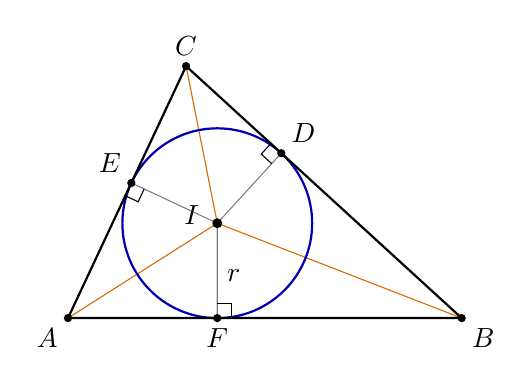
\begin{tikzpicture}[thick]
  % I = (aA + bB + cC) / (a + b + c) = (1.8959, 1.2051) and r = area / s = 1.2051; D, E, F are the feet of the perpendiculars from I
  \coordinate[label=below left:$A$] (A) at (0,0);
  \coordinate[label=below right:$B$] (B) at (5,0);
  \coordinate[label=above:$C$] (C) at (1.5,3.2);
  \coordinate (I) at (1.8959,1.2051);
  \coordinate[label=above right:$D$] (D) at (2.7091,2.0946);
  \coordinate[label=above left:$E$] (E) at (0.8047,1.7166);
  \coordinate[label=below:$F$] (F) at (1.8959,0);
  \draw[orange!85!black, thin] (A) -- (I) (B) -- (I) (C) -- (I);
  \draw[blue!70!black] (I) circle (1.2051);
  \draw (A) -- (B) -- (C) -- cycle;
  \draw[gray, thin] (I) -- (D) (I) -- (E) (I) -- node[right, pos=0.55, black] {$r$} (F);
  \pic[draw, thin, angle radius=1.8mm] {right angle=I--F--B};
  \pic[draw, thin, angle radius=1.8mm] {right angle=I--D--C};
  \pic[draw, thin, angle radius=1.8mm] {right angle=I--E--A};
  \fill (I) circle (1.8pt) node[left=3pt, yshift=3pt] {$I$};
  \foreach \p in {A, B, C, D, E, F} \fill (\p) circle (1.5pt);
\end{tikzpicture}
